\chapter{Кинетическая энергия механической системы. Теорема Кёнига. Теорема об
изменении кинетической энергии механической системы. Закон сохранения
полной механической энергии.}

Кинетической энергией механической системы называется сумма кинетических энергий
всех точек, входящих в систему: \( \ds T = \sum_{j=1}^N T_j \).

\section{Теорема Кёнига}
\begin{table}[h!]
\begin{tabular}{C{.4}m{.55\textwidth}}
    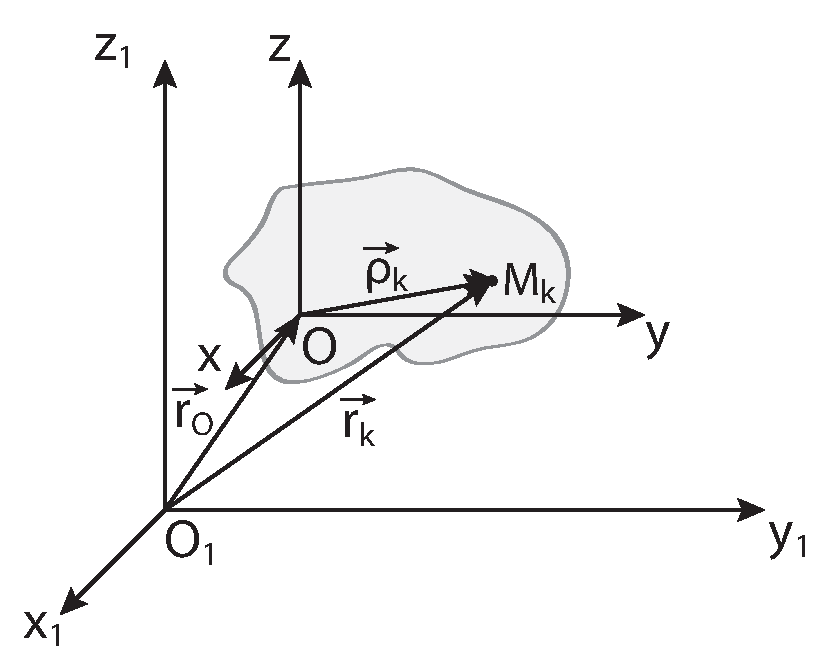
\includegraphics[width=.4\textwidth]{38_01} &
    Рассмотрим две системы отсчёта: неподвижную \( O_1x_1y_1z_1 \) и подвижную
    \( Oxyz \), поступательно движущуюся со скоростью \( \vec{v} \) относительно
    неподвижной.

    Скорость точки \( M_j \) механической системы складывается из её скорости
    относительно движущейся системы отсчёта \( \vec{v}_{jr} \) и скорости
    движущейся системы отсчёта относительно неподвижной:
    \( \vec{v}_j = \vec{v} + \vec{v}_{jr} \).

Тогда кинетическая энергия системы:
\end{tabular}
\end{table}
\vspace*{-2.5em}
\[
    T = \frac{1}{2}\sum_{j=1}^N m_j(\vec{v} + \vec{v}_{jr})^2 = \frac{1}{2}
    \sum_{j=1}^N m_j\vec{v}^2 + \sum_{j=1}^N m_j\vec{v}\cdot\vec{v}_{jr} +
    \frac{1}{2}\sum_{j=1}^N m_j\vec{v}_{jr}^2.
\]

Последняя сумма равна кинетической энергии относительного движения \( T_r \).
Тогда:
\[
    T = \frac{1}{2}\vec{v}^2\sum_{j=1}^N m_j +
    \vec{v}\cdot\sum_{j=1}^Nm_j\vec{v}_{jr} + T_r =
    \frac{1}{2}M\vec{v}^2 + \vec{v}\cdot\sum_{j=1}^N m_j\vec{v}_{jr} + T_r.
\]

Если начало подвижных осей \( O \) совпадает с центром масс \( C \) системы, то
\[
    \sum_{j=1}^N m_j\vec{v}_{jr} = \sum_{j=1}^N m_j\der{\vec{\rho}_j}{t} =
    \der{}{t}\sum_{j=1}^N m_j\vec{\rho}_j = 0.
\]
Значит, кинетическая энергия механической системы:
\( \ds T = \frac{1}{2}M\vec{v}_c^2 + T_c \).

Кинетическая энергия материальной системы равна кинетической энергии в
поступательном движении вместе с центром масс и кинетической энергией в
относительном движении относительно центра масс.

\section{Теорема об изменении кинетической энергии}
Для каждой точки материальной системы будет справедливо следующее:
\[
    \frac{m_j\vec{v}_j^2}{2} - \frac{m_j\vec{v}_{0j}^2}{2} = A^e_j + A^i_j,
\]
где \( A^e_j \) и \( A^i_j \) -- работа внешних и внутренних сил соответственно.

Тогда для всей системы имеем:
\[
    \frac{1}{2}\sum_{j=1}^N m_j\vec{v}_j^2 -
    \frac{1}{2}\sum_{j=1}^N m_j\vec{v}_{0j}^2 =
    \sum_{j=1}^N A^e_j + \sum_{j=1}^N A^i_j, \quad \text{или} \quad
    T - T_0 = A^e + A^i = A.
\]
Изменение кинетической энергии материальной системы при переходе её из
начального в текущее (конечное) положение равно сумме работ на этом перемещении
всех внешних и внутренних сил, приложенных к точкам системы.

\section{Закон сохранения полной механической энергии}
Так как \( A = \varPi_0 - \varPi \) и \( T - T_0 = A \), то \( T_0 - T =
\varPi_0 - \varPi \) или \( T + \varPi = h \), где \( h = T_0 + \varPi_0 =
\const \).
Таким образом, если система движется под действием только консервативных сил, то
сумма кинетической и потенциальной энергий сохраняет постоянное значение.

\newpage
